\documentclass[12pt,a4paper]{article}

\hoffset -1cm
\oddsidemargin 2pt
\headheight 0pt
\headsep 0pt
\topmargin 0pt
\textwidth 18cm 
\textheight 22cm
\usepackage{parskip}
\setlength{\parindent}{15pt}

\usepackage[utf8]{inputenc}
\usepackage[T1]{fontenc}
\usepackage[spanish]{babel}
\usepackage{lmodern}
\usepackage{tikz}
\usetikzlibrary{babel}
%o \usepackage[spanish,mexico]{babel}
\usepackage{microtype}
\usepackage{amsmath,amsthm,amssymb,mathrsfs} %para matematicas
%\usepackage{lipsum}
\usepackage{graphicx}
\usepackage{relsize}
\DeclareGraphicsExtensions{.bmp,.png,.pdf,.jpg}
\usepackage{float}
\spanishdecimal{.}
\newcommand{\N}{\mathbf{N}}
\newcommand{\Z}{\mathbf{Z}}
\newcommand{\Q}{\mathbf{Q}}
\newcommand{\R}{\mathbf{R}}
\newcommand{\C}{\mathbf{C}}
\newcommand{\B}{\mathbf{B}}
\newcommand{\p}{\mathbf{P}}
\newcommand{\E}{\mathbf{E}}

\newcommand{\parentheses}[1]{\left(#1\right)}
\newcommand{\bracket}[1]{\left[#1\right]}
\newcommand{\braces}[1]{\left\{#1\right\}}
\newcommand{\chevrons}[1]{{\left\langle #1\right\rangle }}
\newcommand{\norm}[1]{{\lVert#1\rVert}}
\newcommand{\abs}[1]{{\left|#1\right|}}
\newcommand{\bb}[1]{\mathbb{#1}}

\newtheorem{theorem}{Teorema}
\newtheorem{example}{Ejemplo}
\newtheorem{corollary}{Corolario}[theorem]
\newtheorem{lemma}{Lema}
\newtheorem{exercise}{Ejercicio}
\newtheorem{remark}{Observación}

\theoremstyle{definition}
\newtheorem{definition}{Definición}

\title{Examen Parcial II\\
	\textbf{Procesos Estocásticos I}}
\author{\small{Prof. Rafael Miranda Cordero \hspace{4 cm} Aydte. Fernando Avitúa Varela}}
\date{26 de octubre 2023}
\begin{document}
	\maketitle
	
	Responda 3 de los siguientes problemas. Argumente cuidadosamente sus respuestas. 
	
	\begin{enumerate}
		\item Dé un ejemplo de una cadena de Markov irreducible y transitoria.
		
		\item Diga si los siguientes enunciados son verdaderos o falsos. Argumente su respuesta.
		
		\begin{enumerate}
			\item Una cadena de Markov con espacio de estados finito puede tener todos sus estados transitorios.
			\item Una cadena de Markov con espacio de estados finito siempre tiene al menos un distribución estacionaria.
			\item Los estados recurrentes nulos solo pueden existir en cadenas de Markov con espacio de estados infinito.
		\end{enumerate}
	
		\item Considere una cadena de Markov sobre $S=\braces{0,1,2,3,4,5}$ con matriz de transición dada por
		\begin{equation*}
			\parentheses{\begin{array}{cccccc}
					1 & 0 & 0 & 0 & 0 & 0\\
					1/4 & 1/2 & 1/4 & 0 & 0 & 0 \\
					0 & 1/5 & 2/5 & 1/5 & 0 & 1/5\\
					0 & 0 & 0 & 1/3 & 1/3 & 1/3\\
					0 & 0 & 0 & 1/2 & 0 & 1/2\\
					0 & 0 & 0 & 1/4 & 0 & 3/4\\
			\end{array}}
		\end{equation*}
		determine las clases de comunicación de la cadena. 
		\begin{enumerate}
			\item Determine cuales clases son de transitorios y cuales son de recurrentes.
			\item Calcule las probabilidades de absorición de los estados transitorios.
			\item Calcule las distribuciones estacionarias concentradas en las clases de comunicación de recurrentes.
		\end{enumerate}
		
		\item (Repair Chain). Una maquina tiene tres piezas que son críticas para su funcionamiento y son susceptibles a fallar, no obstante la maquina puede continuar funcionando siempre y cuando dos de estas piezas continúen trabajando. Cuando dos pieza se rompen, ellas son reemplazadas y la maquina regresa a sus funciones usuales al día siguiente. Considere $X_n$ la variable aleatoria que nos dice cuales piezas están rotas en el día $n$, es decir, si las piezas las numeramos como 1,2 y 3, entonces $X_n$ toma el valor $0$ si ninguna pieza esta fallando, el valor $i$ si la pieza  rota es la pieza $i=1,2,3$ y es la única pieza rota ese día, el valor $12$ (entiéndase como 1-2) si las piezas 1 y 2 están fallando ese día y lo análogo para los valores $13$ (1-3) y $23$ (2-3). Asumimos que las piezas 1, 2 y 3 pueden fallar con probabilidad $0.01$, $0.02$ y $0.04$ respectivamente, pero que no pueden fallar dos el mismo día. En este contexto, la colección $\braces{X_n:n\geq 0}$ puede ser considerada una cadena de Markov con espacio de estados $S=\braces{0,1,2,3,12,13,23}$ y matriz de transición como la de la figura 1. Si operaremos la máquina por 1,800 días (cerca de 5 años) ¿aproximadamente cuantas piezas del tipo 1, 2 y 3 usaremos?
		
		\emph{Sugerencia:} Utilice el hecho que $N_n(y)/n\rightarrow 1/m_y \text{  c.s.}$ como $n\rightarrow \infty$ si $y$ es recurrente positivo.
		\begin{figure}[H]
			\centering
			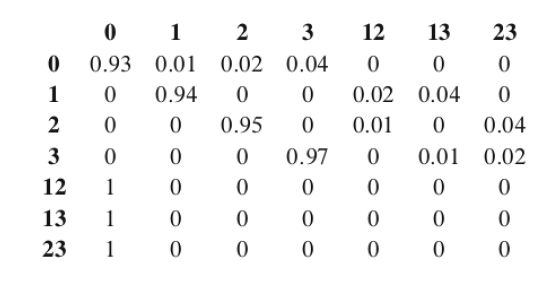
\includegraphics[width=0.6\linewidth]{ej6.png}
			\caption{}
			\label{fig:exampl17durret}
		\end{figure}
	
	\end{enumerate}

	
\end{document}